\documentclass[tikz,border=8pt]{standalone}
\usepackage{tikz}
\usepackage{amssymb}
\usetikzlibrary{shapes.geometric, arrows.meta, positioning, calc}
\definecolor{pbblue}{HTML}{E6F3FF}
\definecolor{pbdarkblue}{HTML}{1E3A8A}
\definecolor{pbmint}{HTML}{E0F2F1}
\definecolor{pbdarkgreen}{HTML}{065F46}
\definecolor{pblavender}{HTML}{F3E5F5}
\definecolor{pbdarkpurple}{HTML}{581C87}
\definecolor{pbyellow}{HTML}{FEF3C7}
\definecolor{pbcoral}{HTML}{FEE2E2}
\definecolor{pbdarkred}{HTML}{991B1B}
\definecolor{pbgray}{HTML}{F3F4F6}

\begin{document}
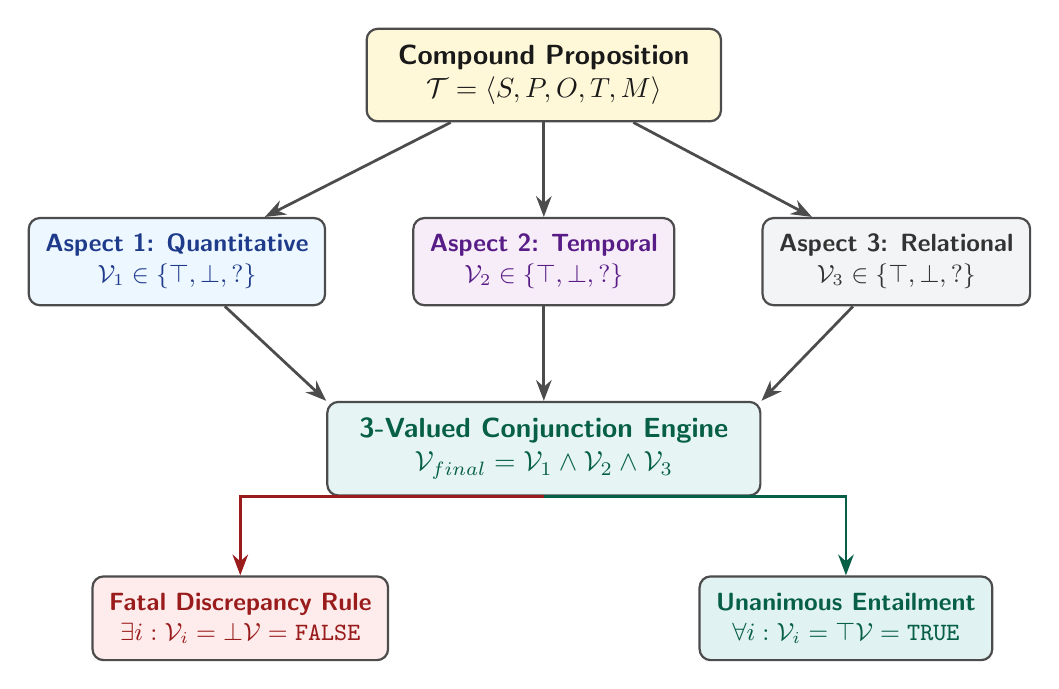
\begin{tikzpicture}[
    font=\sffamily\small,
    box/.style={draw=black!70, rounded corners=4pt, line width=0.8pt, align=center, inner sep=6pt},
    arrow/.style={-{Stealth[scale=1.0]}, line width=1pt, draw=black!70}
]

\node[box, fill=pbyellow!70, text=black!90, font=\bfseries\sffamily, minimum width=4.5cm] (input) {Compound Proposition\\$\mathcal{T} = \langle S, P, O, T, M \rangle$};

\node[box, fill=pbblue!70, text=pbdarkblue, below left=1.2cm and 0.5cm of input, minimum width=3.2cm] (m1) {\textbf{Aspect 1: Quantitative}\\$\mathcal{V}_1 \in \{\top, \bot, ?\}$};
\node[box, fill=pblavender!70, text=pbdarkpurple, below=1.2cm of input, minimum width=3.2cm] (m2) {\textbf{Aspect 2: Temporal}\\$\mathcal{V}_2 \in \{\top, \bot, ?\}$};
\node[box, fill=pbgray, text=black!80, below right=1.2cm and 0.5cm of input, minimum width=3.2cm] (m3) {\textbf{Aspect 3: Relational}\\$\mathcal{V}_3 \in \{\top, \bot, ?\}$};

\draw[arrow] (input) -- (m1);
\draw[arrow] (input) -- (m2);
\draw[arrow] (input) -- (m3);

\node[box, fill=pbmint!80, text=pbdarkgreen, font=\bfseries\sffamily, below=1.2cm of m2, minimum width=5.5cm] (dag) {3-Valued Conjunction Engine\\$\mathcal{V}_{\text{final}} = \mathcal{V}_1 \wedge \mathcal{V}_2 \wedge \mathcal{V}_3$};

\draw[arrow] (m1) -- (dag.north west);
\draw[arrow] (m2) -- (dag.north);
\draw[arrow] (m3) -- (dag.north east);

\node[box, fill=pbcoral!70, text=pbdarkred, below left=1.0cm and -0.8cm of dag, minimum width=3.5cm] (rule1) {\textbf{Fatal Discrepancy Rule}\\$\exists i: \mathcal{V}_i = \bot \implies \mathcal{V} = \texttt{FALSE}$};
\node[box, fill=pbmint, text=pbdarkgreen, below right=1.0cm and -0.8cm of dag, minimum width=3.5cm] (rule2) {\textbf{Unanimous Entailment}\\$\forall i: \mathcal{V}_i = \top \implies \mathcal{V} = \texttt{TRUE}$};

\draw[arrow, draw=pbdarkred] (dag.south) -| (rule1.north);
\draw[arrow, draw=pbdarkgreen] (dag.south) -| (rule2.north);

\end{tikzpicture}
\end{document}